\chapter{الضوء والظلال}\label{ch:g1:light-and-shadows}

أطفئ المصباح في غرفة بلا نافذة: يختفي كل شيء. أشعله: تعود الغرفة.
الرؤية تحتاج إلى \omterm{def:g1:light-and-shadows:source}{ضوء}. وحيثما كان \omterm{def:g1:light-and-shadows:source}{ضوء} كانت ظلال --- فتوأمك المعتم
الوفيّ يتبعك على كل رصيف مشمس. فلنكتشف من أين يأتي \omterm{def:g1:light-and-shadows:source}{الضوء}، وكيف
تُصنع الظلال.

\section{من أين يأتي الضوء}

\begin{definition}[منابع الضوء]\label{def:g1:light-and-shadows:source}
\emph{منبع الضوء}\index{منبع ضوء} شيء يصنع \emph{ضوءه}\index{ضوء}
بنفسه: الشمس، والمصباح، ولهب الشمعة، واليراعة. أما كل ما عدا ذلك
--- كتاب، وكرة، وجدران، وأنت --- فلا يصنع ضوءًا خاصًّا به: ولا
نرى هذه الأشياء إلا حين يقع عليها ضوء من منبع.
\end{definition}

\begin{example}[منابع أم لا؟]\label{ex:g1:light-and-shadows:sources}
الشمس، والمصباح اليدوي، وعود الثقاب المشتعل، وشاشة التلفاز، كلها
تصنع ضوءًا: فهي منابع. أما القمر والمرآة والجدار الأبيض فقد تبدو
شديدة السطوع، لكنها لا تصنع ضوءًا خاصًّا بها --- إنما تردّ \omterm{def:g1:light-and-shadows:source}{الضوء}
الذي يصلها. أطفئ المصباح، فأشدّ المرايا سطوعًا يغرق في العتمة.
\end{example}

\begin{example}[جرّب: الغرفة المعتمة]\label{ex:g1:light-and-shadows:darkroom}
في المساء، أغلق مصاريع غرفة أو ستائرها، وأطفئ كل مصباح، وانتظر
وأنت تعدّ على مهل حتى $20$. ماذا ترى؟ لا شيء تقريبًا في البداية
--- فبلا منبع لا \omterm{def:g1:light-and-shadows:source}{ضوء} يُرى به. ثم افتح الباب قليلًا: شريحة \omterm{def:g1:light-and-shadows:source}{ضوء}
رفيعة واحدة تكفي لإعادة الطاولات والكراسي والألعاب.
\end{example}

\begin{remark}[لا تنظر إلى الشمس أبدًا]\label{rem:g1:light-and-shadows:sun}
الشمس أقوى \omterm{def:g1:light-and-shadows:source}{منبع ضوء} نلقاه على الإطلاق. لا تنظر إليها مباشرة أبدًا،
ولا للحظة واحدة، ولا عبر منظار أو عدسة مكبّرة: ضوءها من القوة بحيث
يؤذي عينيك أذًى دائمًا. إنما تُستمتع الشمس من جانبها --- \omterm{def:g1:light-and-shadows:source}{بالضوء}
الذي تلقيه على كل ما سواها.
\end{remark}

\section{كيف تُصنع الظلال}

\begin{definition}[الظلّ]\label{def:g1:light-and-shadows:shadow}
\emph{الظلّ}\index{ظلّ} هو الرقعة المعتمة التي تظهر خلف شيء يحجب
\omterm{def:g1:light-and-shadows:source}{الضوء}. \omterm{def:g1:light-and-shadows:source}{فالضوء} لا ينفذ من جسمك، ولذلك لا تنال الأرض خلفك ضوءًا من
الشمس: تلك الرقعة المعتمة التي على شكلك هي ظلّك.
\end{definition}

\begin{omfigure}
\begin{tikzpicture}[scale=0.85]
  % two rays from the lamp, exactly tangent to the ball (computed:
  % source (0,1.5), ball center (4.2,1.5), r=0.55 -> wall hits y=1.5±1.004)
  \draw[omThm] (0,1.5) -- (7.6,2.504);
  \draw[omThm] (0,1.5) -- (7.6,0.496);
  % free rays that miss the ball entirely
  \draw[omThm] (0,1.5) ++(32:0.42) -- ++(32:2.4);
  \draw[omThm] (0,1.5) ++(-32:0.42) -- ++(-32:2.4);
  \fill[omThm] (0,1.5) circle (0.3);
  \draw[thick, fill=omDef, fill opacity=0.3] (4.2,1.5) circle (0.55);
  \draw[very thick] (7.6,-0.4) -- (7.6,3.4);
  \draw[line width=3.5pt, omExo] (7.6,0.496) -- (7.6,2.504);
  \node[below, font=\small] at (0,1.0) {مصباح};
  \node[below, font=\small] at (4.2,0.7) {كرة};
  \node[right, font=\small] at (7.75,1.5) {ظلّ};
  \node[right, font=\small] at (7.75,3.0) {جدار};
\end{tikzpicture}

{\small المصباح يضيء، والكرة تحجب، والجدار خلفها يبقى معتمًا:
مصباح، فحاجب، \omterm{def:g1:light-and-shadows:shadow}{فظلّ} --- بهذا الترتيب دائمًا، وعلى استقامة واحدة.}
\end{omfigure}

\begin{method}[كيف تصنع ظلًّا حادًّا]\label{met:g1:light-and-shadows:make}
\begin{enumerate}
  \item أعتِم الغرفة --- فالظلال تختبئ حين يأتي \omterm{def:g1:light-and-shadows:source}{الضوء} من كل
        مكان؛
  \item أشعل مصباحًا \emph{واحدًا} أو مصباحًا يدويًّا؛
  \item ضع لعبة بين المصباح والجدار؛
  \item انظر إلى الجدار: هناك \omterm{def:g1:light-and-shadows:shadow}{الظلّ}، في الجهة البعيدة من اللعبة
        عن المصباح.
\end{enumerate}
قرّب اللعبة من المصباح: يكبر \omterm{def:g1:light-and-shadows:shadow}{الظلّ} كبرًا هائلًا. وقرّبها من
الجدار: يتقلّص \omterm{def:g1:light-and-shadows:shadow}{الظلّ} إلى حجم اللعبة الحقيقي.
\end{method}

\begin{example}[جرّب: حيوانات من ظلّ]\label{ex:g1:light-and-shadows:animals}
بالمصباح نفسه في \cref{met:g1:light-and-shadows:make}، ضع يديك في
\omterm{def:g1:light-and-shadows:source}{الضوء} بدل اللعبة: إصبعان مرفوعتان تصنعان أذنَي أرنب، وإبهامان
متقاطعان يصنعان طائرًا يطير. يُظهر الجدار الشكل الذي اقتطعته يداك
من \omterm{def:g1:light-and-shadows:source}{الضوء} --- \omterm{def:g1:light-and-shadows:shadow}{والظلّ} يحفظ دائمًا شكل حاجبه كما يُرى من المصباح.
\end{example}

\begin{remark}[الظلّ ليس شيئًا]\label{rem:g1:light-and-shadows:notathing}
لا تستطيع أن تلتقط ظلًّا، ولا أن تطويه، ولا أن تحفظه في علبة.
\omterm{def:g1:light-and-shadows:shadow}{فالظلّ} ليس مصنوعًا من شيء: إنما هو \emph{موضع غاب عنه \omterm{def:g1:light-and-shadows:source}{الضوء}}.
ولهذا يتلاشى لحظة انطفاء المصباح --- إذ ليس هناك شيء يبقى.
\end{remark}

\section{الظلال تتبع الضوء}

\begin{example}[في أيّ جهة الظلّ؟]\label{ex:g1:light-and-shadows:opposite}
في الصباح تكون الشمس في جهة منك ويقع ظلّك في الجهة \emph{الأخرى}.
واجه الشمس: يختبئ ظلّك خلفك. وأدر ظهرك للشمس: يمتدّ ظلّك أمامك.
\omterm{def:g1:light-and-shadows:shadow}{الظلّ} يقع دائمًا في الجهة المقابلة للمنبع تمامًا.
\end{example}

\begin{omfigure}
\begin{tikzpicture}[scale=0.75]
  % low sun: the ray from the Sun grazing the stick's tip is drawn
  % straight; the shadow ends exactly where that ray meets the ground
  % (sun (0.7,2.2), tip (3.4,1.2) -> ground at x=6.64)
  \fill[omThm] (0.7,2.2) circle (0.4);
  \foreach \a in {0,45,...,315} {
    \draw[omThm] (0.7,2.2) ++(\a:0.55) -- ++(\a:0.25);
  }
  \draw[omThm] (0.7,2.2) -- (6.64,0);
  \draw[line width=2.6pt] (3.4,0) -- (3.4,1.2);
  \draw[thick] (2.2,0) -- (7.0,0);
  \draw[line width=3.5pt, omExo] (3.4,-0.09) -- (6.64,-0.09);
  \node[below, font=\small] at (4.6,-0.35) {شمس منخفضة: ظلّ طويل};
  % high sun: same stick, the grazing ray is steep
  % (sun (8.6,3.6), tip (10.2,1.2) -> ground at x=11.0)
  \fill[omThm] (8.6,3.6) circle (0.4);
  \foreach \a in {0,45,...,315} {
    \draw[omThm] (8.6,3.6) ++(\a:0.55) -- ++(\a:0.25);
  }
  \draw[omThm] (8.6,3.6) -- (11.0,0);
  \draw[line width=2.6pt] (10.2,0) -- (10.2,1.2);
  \draw[thick] (9.0,0) -- (11.8,0);
  \draw[line width=3.5pt, omExo] (10.2,-0.09) -- (11.0,-0.09);
  \node[below, font=\small] at (10.4,-0.35) {شمس عالية: ظلّ قصير};
\end{tikzpicture}

{\small العصا نفسها، صباحًا وظهرًا. ينتهي \omterm{def:g1:light-and-shadows:shadow}{الظلّ} حيث يلتقي بالأرض
الشعاعُ المستقيم المارّ بطرف العصا: فالشمس المنخفضة تمدّه طويلًا،
والشمس العالية تقبضه قصيرًا.}
\end{omfigure}

\begin{omfigure}
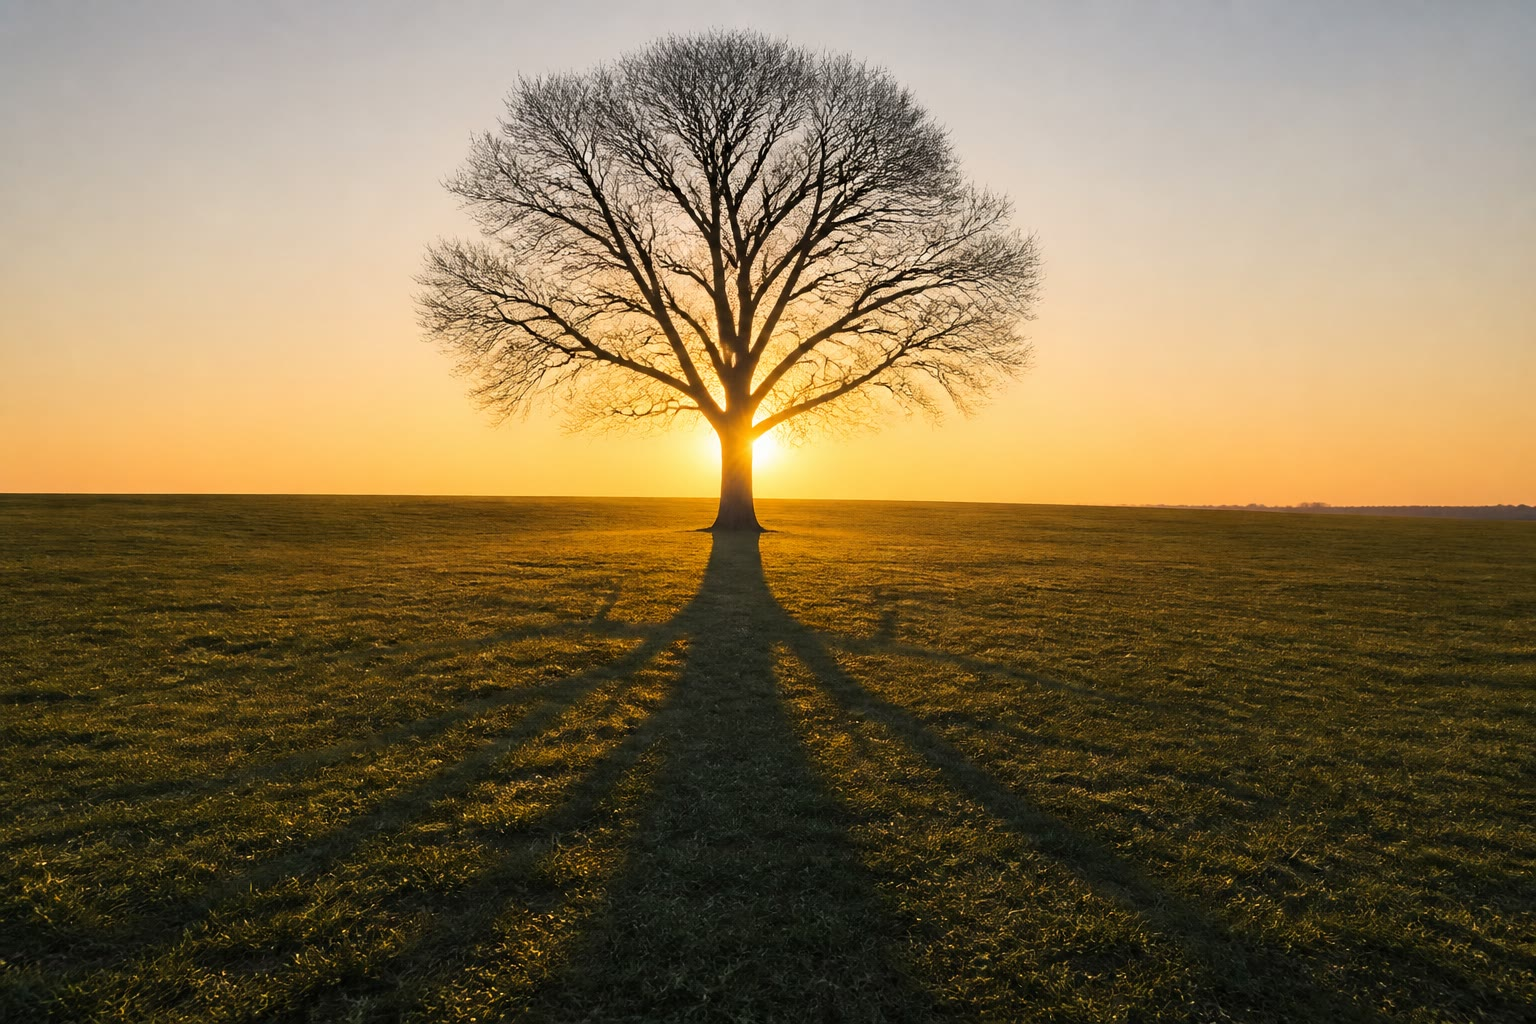
\includegraphics[width=0.6\linewidth]{images/book1/ai/g1-light-shadows-long-shadow.jpg}

{\small شمس مسائية منخفضة \omterm{def:g1:light-and-shadows:shadow}{وظلّ} طويل: كلما انخفضت الشمس امتدّ كل \omterm{def:g1:light-and-shadows:shadow}{ظلّ} أبعد.}
\end{omfigure}

\begin{example}[جرّب: طباشير حول ظلّ]\label{ex:g1:light-and-shadows:chalk}
في صباح مشمس، قف ساكنًا في الساحة بينما يرسم صديقك خطًّا بالطباشير
حول ظلّك. ثم عُد بعد الغداء وقف في الموضع نفسه: لقد خرج ظلّك من
خطّ الطباشير وتغيّر طوله! لقد غيّرت الشمس موضعها في السماء ---
فتبعها \omterm{def:g1:light-and-shadows:shadow}{الظلّ}. والفصل التالي يتبع الشمس في يومها كله.
\end{example}

\section{تمارين}

\begin{exercise}[$\star$]\label{exo:g1:light-and-shadows:1}
صنّف إلى منابع \omterm{def:g1:light-and-shadows:source}{ضوء} وغير منابع: لهب شمعة؛ \ القمر؛
\ يراعة؛ \ مرآة؛ \ مصباح يدوي؛ \ جدار أبيض.
\end{exercise}

\begin{exercise}[$\star$]\label{exo:g1:light-and-shadows:2}
لماذا لا ترى شيئًا البتة في غرفة مغلقة بلا نافذة ولا مصباح؟ ما
الذي ينقصها؟
\end{exercise}

\begin{exercise}[$\star$]\label{exo:g1:light-and-shadows:3}
سمِّ الأشياء الثلاثة اللازمة لصنع \omterm{def:g1:light-and-shadows:shadow}{ظلّ} على الجدار، ورتّبها الترتيب
الصحيح على استقامة واحدة.
\end{exercise}

\begin{exercise}[$\star$]\label{exo:g1:light-and-shadows:4}
الشمس عن يسارك. في أيّ جهة ظلّك؟ ثم استدرتَ فصرت تواجه الجهة
المعاكسة --- أين هو الآن؟
\end{exercise}

\begin{exercise}[$\star$]\label{exo:g1:light-and-shadows:5}
باستعمال \cref{met:g1:light-and-shadows:make}، اجعل \omterm{def:g1:light-and-shadows:shadow}{ظلّ} اللعبة
نفسها هائلًا أولًا ثم صغيرًا. ما الذي حرّكته، وفي أيّ اتجاه؟
\end{exercise}

\begin{exercise}[$\star$]\label{exo:g1:light-and-shadows:6}
أيمكن التقاط \omterm{def:g1:light-and-shadows:shadow}{ظلّ} ووضعه في جيب؟ اشرح ما \omterm{def:g1:light-and-shadows:shadow}{الظلّ} حقًّا، مستعينًا
بما في \cref{rem:g1:light-and-shadows:notathing}.
\end{exercise}

\begin{exercise}[$\star$]\label{exo:g1:light-and-shadows:7}
لماذا يجب ألّا تنظر إلى الشمس مباشرة أبدًا، مع أن النظر إلى مصباح
لا يبهرك إلا قليلًا؟
\end{exercise}

\begin{exercise}[$\star$]\label{exo:g1:light-and-shadows:8}
عند الظهر تعلو الشمس؛ وفي آخر العصر تنخفض. متى يكون ظلّك أطول؟
ارسم ظلَّي شجرة، واحدًا لكل لحظة.
\end{exercise}

\begin{exercise}[$\star\star$]\label{exo:g1:light-and-shadows:9}
تقول ميا: ``كان ظلّي أمامي، وبعد أن استدرت صار خلفي --- إذن
استدار \omterm{def:g1:light-and-shadows:shadow}{الظلّ} معي.'' ويقول سام إن \omterm{def:g1:light-and-shadows:shadow}{الظلّ} لم يتحرّك البتة. فكّر في
\cref{ex:g1:light-and-shadows:opposite}: مَن المصيب، ولماذا
\emph{بدا} أن \omterm{def:g1:light-and-shadows:shadow}{الظلّ} استدار؟
\end{exercise}
